% Global document settings
\documentclass[10pt]{article}

% Packages
\usepackage{tgtermes}
\usepackage{graphicx}
\usepackage{natbib}
\usepackage{authblk}
\usepackage{array}
\usepackage{colortbl}
\usepackage{tocloft}
\usepackage{xcolor}
\usepackage{siunitx}
\usepackage{setspace}
\usepackage{listings}
\usepackage{caption}
\usepackage[T1]{fontenc}
\usepackage[nottoc]{tocbibind}
\usepackage[breaklinks]{hyperref}
\usepackage[font=small,skip=7pt]{caption}

% Custom colours
\definecolor{codegreen}{rgb}{0,0.6,0}
\definecolor{codegray}{rgb}{0.5,0.5,0.5}
\definecolor{codepurple}{rgb}{0.58,0,0.82}
\definecolor{backcolour}{rgb}{0.95,0.95,0.92}

% Listing styles
\lstdefinestyle{mystyle}{
  backgroundcolor=\color{backcolour},
  commentstyle=\color{codegreen},
  keywordstyle=\color{purple},
  numberstyle=\tiny\color{codegray},
  stringstyle=\color{codepurple},
  basicstyle=\ttfamily\footnotesize,
  breakatwhitespace=false,
  breaklines=true,
  captionpos=b,
  keepspaces=true,
  numbers=left,
  numbersep=5pt,
  showspaces=false,
  showstringspaces=true,
  showtabs=false,
  tabsize=2
  }
  \lstset{style=mystyle}

  % Custom commands
  \renewcommand{\bibname}{References} % Change bibliography title
  \renewcommand\cftsecafterpnum{\vskip8pt}
  \renewcommand{\lstlistlistingname}{List of \lstlistingname s}
  \renewcommand{\bibsection}{\section*{Bibliography}}
  \renewcommand{\contentsname}{Table of Contents}
  \renewcommand{\bibsection}{\section{\bibname}}
  \renewcommand{\cftsecleader}{\cftdotfill{\cftdotsep}}

  % Custom settings
  \captionsetup{justification=centering}
  \PassOptionsToPackage{hyphens}{url}
  \urlstyle{same}
  \def\Urlmuskip{0mu}
  \def\UrlBreaks{\do\/\do-}
  \hypersetup{
    colorlinks = true,
    urlcolor = blue,
    linkcolor = black,
    citecolor = black,
  breaklinks=true,
  pdfpagemode=UseOutlines,
  bookmarksopen=true,
  bookmarksopenlevel=2,
  bookmarksnumbered=true
  }

  \title{\textbf{The Neuroscience of Cultured Meat:}\\ Consumer Adoption and Market Disruption}
  \author[ ]{Daniel Burger}
  \affil[ ]{\textbf{King’s College London}}
  \affil[ ]{\href{mailto:public@danielburger.online}{public@danielburger.online}}
  \date{\textit{10. October 2023}}

\begin{document}
% \pagenumbering{roman}
% \counterwithin{lstlisting}{section}
% \counterwithin{figure}{section}
% \counterwithin{table}{section}

\maketitle
% \thispagestyle{empty}

% Double spacing for feedback
% \doublespacing

\begin{sloppypar} % For better line breaks
  \begin{abstract}
    Lab-grown meat, sometimes called cultured meat, presents a sustainable and ethical alternative to traditional meat, addressing environmental and ethical issues associated with industrial animal agriculture. This essay explores the intersection of neuroscience and consumer adoption in the marketing of lab-grown meat. It examines the potential strategies necessary for consumer adoption, such as replicating the sensory qualities of conventional meat, optimising nutritional content, and ensuring product safety and sustainability. A significant focus is placed on the role of neuromarketing in understanding consumer perceptions and decision-making processes. The essay systematically reviews and discusses recent research employing functional magnetic resonance imaging (fMRI), electroencephalography (EEG) neuroimaging, and eye-tracking techniques to provide neuroscientific insights into consumer behaviour, aiming to enhance the marketing strategies for lab-grown meat to the general public.

    Additionally, the essay considers the broader implications of cultured meat research in related scientific fields, with potential benefits in organ transplantation, drug testing models, and the development of biologically plausible neural tissues.
  \end{abstract}
  \pagebreak

  \pagenumbering{Roman}
  \tableofcontents
  \pagebreak

  \listoffigures
  \pagebreak

  % \listoftables
  % \pagebreak

  % Back to normal numbering
  \pagenumbering{arabic}

  \section{Introduction}
  \label{sec:introduction}

  Generating traditional meat through livestock farming has brought forth prominent discussions regarding its alignment with ecological balance, the global climate scenario, and the ethical treatment of animals. Livestock production is estimated to account for approximately 34\% of global greenhouse gas emissions, requiring large amounts of land, water and feed crops \citep{tuomisto_environmental_2011}. In addition, practices in industrial animal farming such as close confinement in crates and cages, painful mutilations like dehorning, and selective breeding for accelerated growth have faced ethical criticisms regarding infringement of animal rights and natural behaviours \citep{stephens_bringing_2018}. As global meat consumption continues to rise, there is an urgent need for more sustainable and ethical alternatives to conventional meat production.


  % TODO Add a figure (e.g. from Mosa Meat)
  Laboratory-grown meat offers a promising solution to address these issues associated with industrial animal agriculture. It involves growing animal cells in a culture medium rich in nutrients, encouraging them to proliferate and differentiate into muscle and fat tissues \citep{datar_possibilities_2010}, exemplarily shown in Figure XYZ. This emerging technology enables meat production without animal slaughter and with substantially lower greenhouse gas emissions land and water use compared to conventional methods \citep{tuomisto_environmental_2011}. However, optimising bioreactor design and cell culture media formulation by reducing production costs is a crucial barrier to commercialisation \citep{specht_opportunities_2018}.

  Consumer research indicates that concerns about environmental sustainability and animal welfare could motivate the purchase of lab-grown meat as an alternative to traditional meat \citep{circus_exploring_2018}. However, public perceptions and reactions to this novel food technology are still largely unknown and warrant further investigation \citep{verbeke_would_2015}. Consumers may harbour concerns regarding the safety, taste, price and perceived naturalness of lab-grown meat \citep{bryant_consumer_2018}. As we move towards a future where lab-grown meat products will likely become a more prevalent part of the food industry, uncertainties and challenges must be addressed. However, with the help of neuromarketing techniques, we can gain valuable insights into consumer decision-making and emotional responses that can help us overcome these challenges. By better understanding consumers’ motivations, preferences and attitudes, we can develop and market lab-grown meat products more successfully.

  This essay will provide an overview of the role of neuroscientific findings in developing and marketing lab-grown meat. Topics covered will include consumer perceptions, neuromarketing applications, product development strategies, and potential marketing approaches to introduce this sustainable protein alternative.

  \section{How Developing Lab-Grown Meat Works}
  \label{sec:developing-lab-grown-meat}

  Several key factors must be considered in developing high-quality lab-grown meat products that can successfully replace conventional meat. Creating lab-grown meat is a multi-step process that involves cell isolation and others, as illustrated in \autoref{fig:lab-grown-meat-process}.

  \begin{figure}[ht]
    \centering
    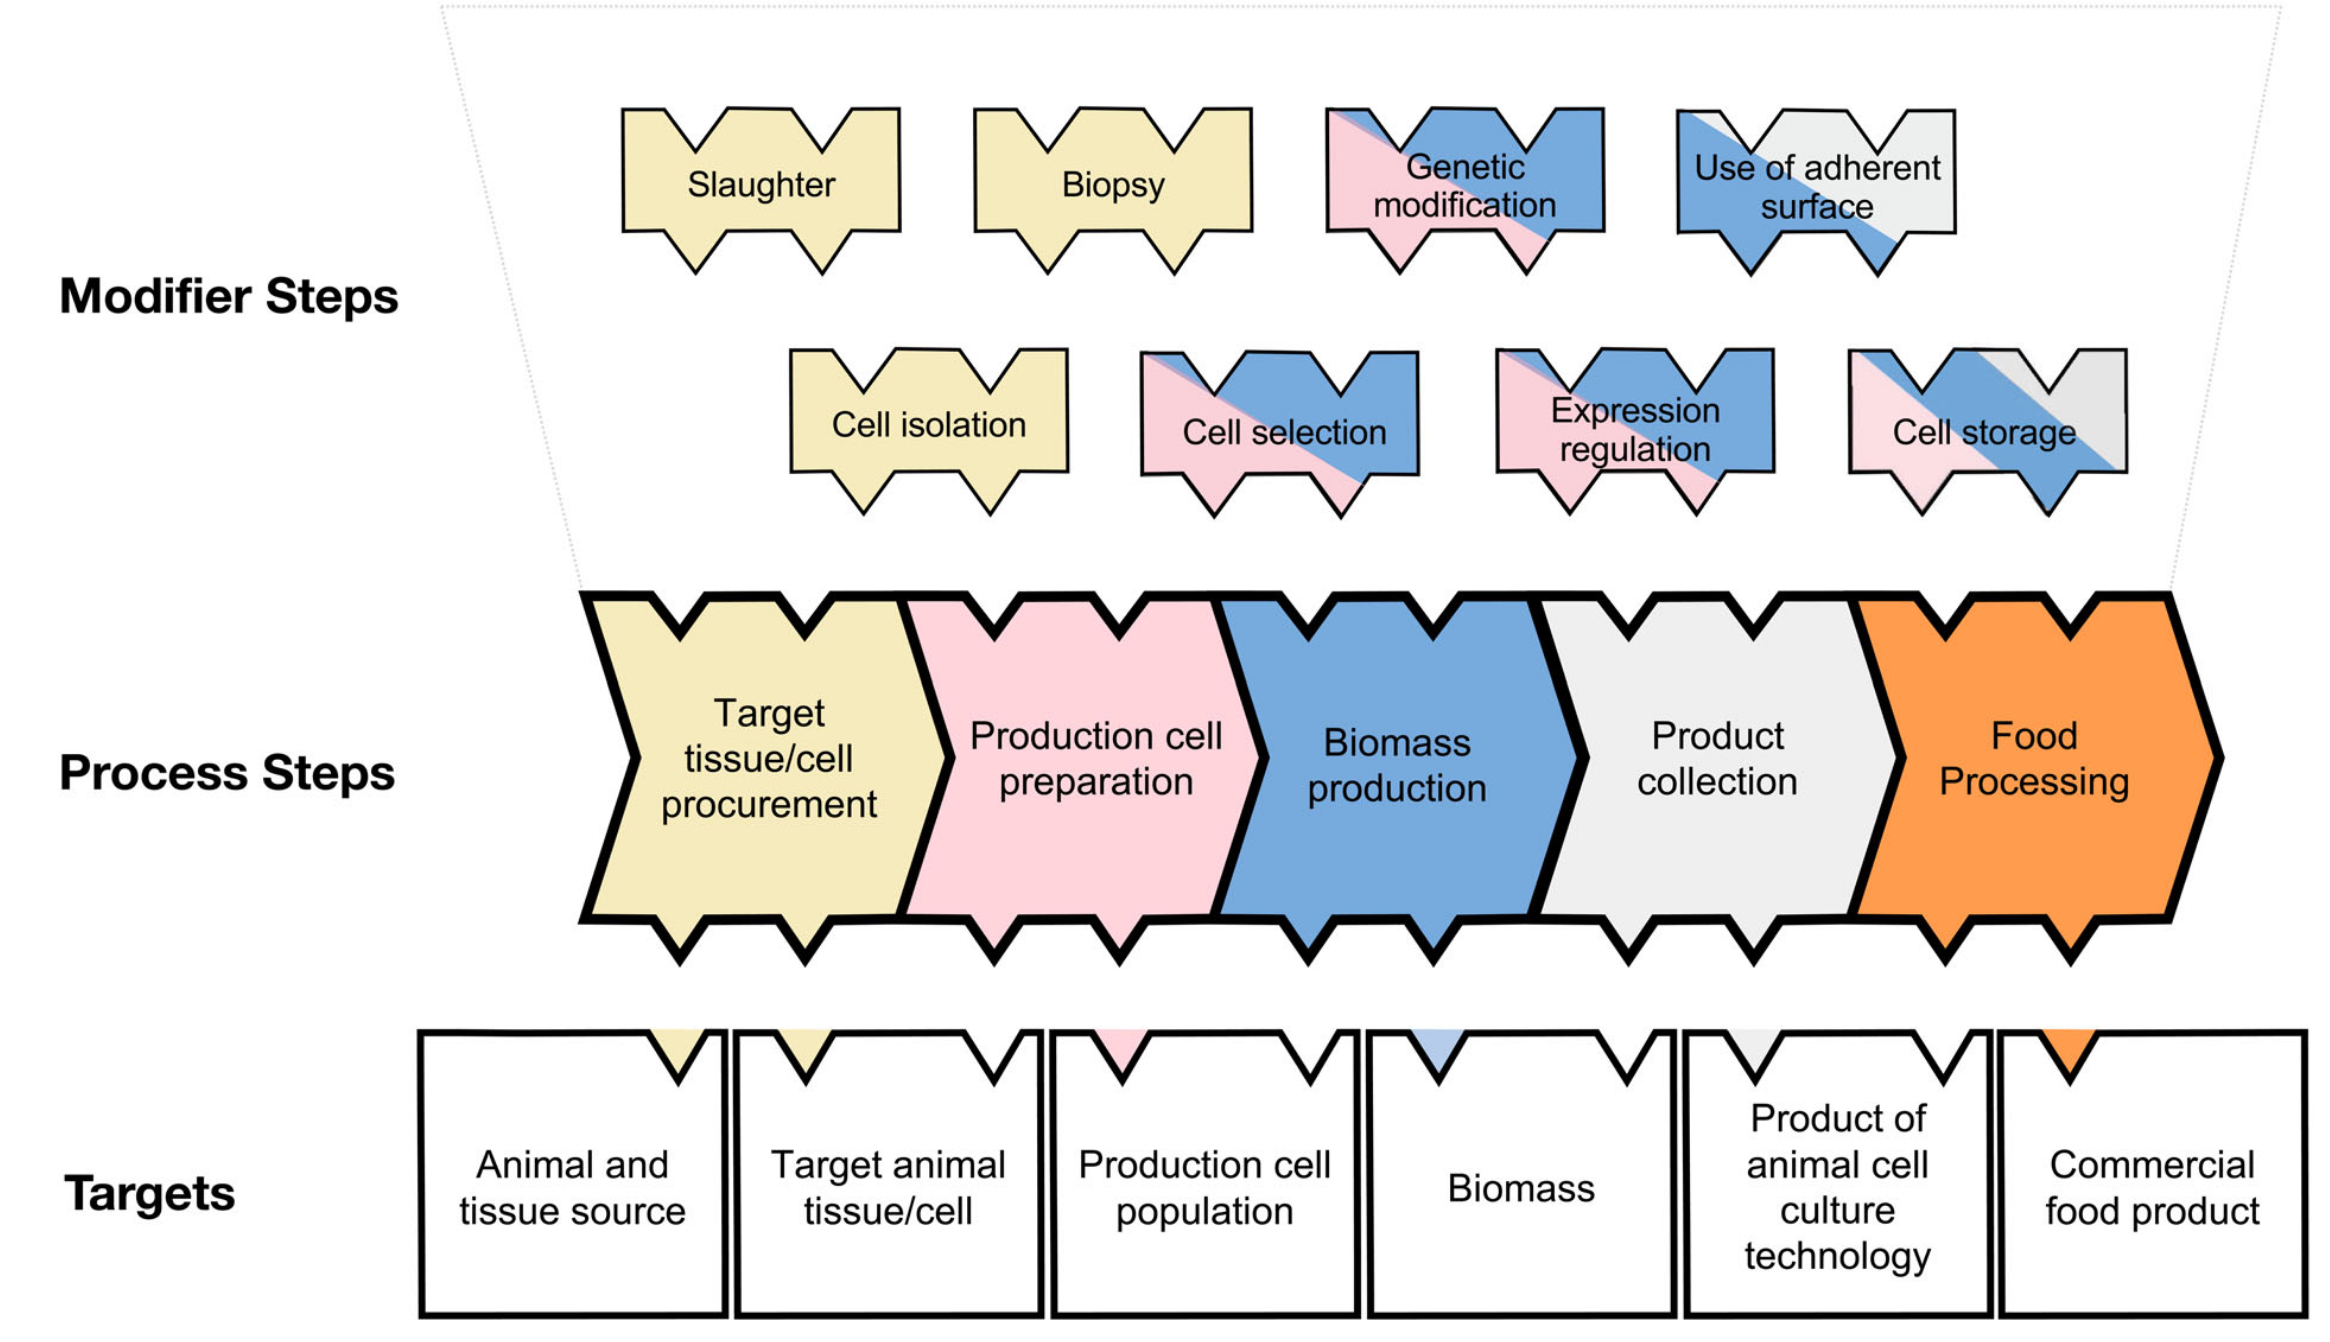
\includegraphics[width=\textwidth]{figures/lab-grown-meat-step.png}
    \caption[Modular process diagram depicting the generalised steps in cultured meat and seafood production.]{\textbf{Modular process diagram depicting the generalised steps in cultured meat and seafood production.} The main steps are obtaining initial cells from an animal source, preparing a cell line through isolation, culture, optimisation and selection, increasing cell biomass via proliferation, differentiation and/or maturation, harvesting the cultured product, and incorporating it into food items. Modifier steps like cell isolation, genetic modification, selection and storage may occur at various points. Arrows indicate the process flow from each step to the next \citep{ong_food_2021}.}
    \label{fig:lab-grown-meat-process}
  \end{figure}

  Texture and mouthfeel are essential attributes, with consumers expecting a comparable experience to cooked animal meat \citep{datar_possibilities_2010}. Culturing techniques that promote muscle fibre alignment and the formation of connective tissue can help achieve the texture profile of whole-cut meats like steak \citep{post_cultured_2012}. For ground products like burgers, smaller tissue spheroids or microcarriers can be used \citep{specht_opportunities_2018}.

  Flavour compounds produced during the cooking process also affect taste and should be matched to traditional meat using ingredients like heme to catalyse reactions like Maillard browning \citep{post_cultured_2012}.

  Ensuring adequate nutritional quality is also critical. Fortification of culture medium with iron, zinc, vitamin B12, and other micronutrients found in meat can optimise the nutritional composition of cultured meat \citep{fraeye_sensorial_2020}. Health claims related to potential benefits like reduced saturated fats may add appeal for some consumers but require scientific substantiation \citep{sergelidis_lab_2019}.

  Rigorous safety testing and compliance with regulatory standards will help address potential consumer concerns and build confidence in lab-grown meat. Careful screening for pathogens and contaminants combined with strict quality control during manufacturing is imperative \citep{ong_food_2021}. Obtaining regulatory approval from the FDA and USDA demonstrates oversight and safety, as it did just some time ago for two companies \citep{mccarthy_usda_nodate}.

  Environmental sustainability of production methods should be demonstrated through life cycle assessments (LCAs) accounting for factors like energy use, emissions and raw material inputs \citep{mattick_anticipatory_2015}. Communicating the results of such studies can reinforce the ecological benefits compared to conventional meat.

  Last but not least, transparent labelling that provides consumers with clear information on lab-grown meat’s origin and production process will be necessary for acceptance and adoption \citep{failla_evaluation_2023}. Descriptive designations help inform purchasing decisions.

  Addressing these areas will allow developers of lab-grown meat to create products that match or exceed traditional meat in terms of sensory factors, nutritional content, safety and sustainability.

  \section{Consumer Perceptions and Attitudes}
  \label{sec:consumer-perceptions-and-attitudes}

  Understanding consumer perceptions, motivations, and potential barriers regarding lab-grown meat is essential for its successful introduction and adoption.

  Qualitative techniques like interviews and focus groups provide deeper insights into consumers’ values, concerns and ambivalence toward lab-grown meat \citep{laestadius_is_2015}. For example, doubts about naturalness and mixed perceptions of high-tech food production emerge in focus groups. Interviews reveal nuanced risk-benefit calculations regarding ethics, environment, and personal health. These methods reveal complex psychological factors shaping attitudes. Cultural and religious values also play a role, as do varying levels of trust in institutions \citep{al-kwifi_dynamics_2019}. Incorporating findings from qualitative research provides a more complete understanding of consumer decision-making.

  \begin{figure}[ht]
    \centering
    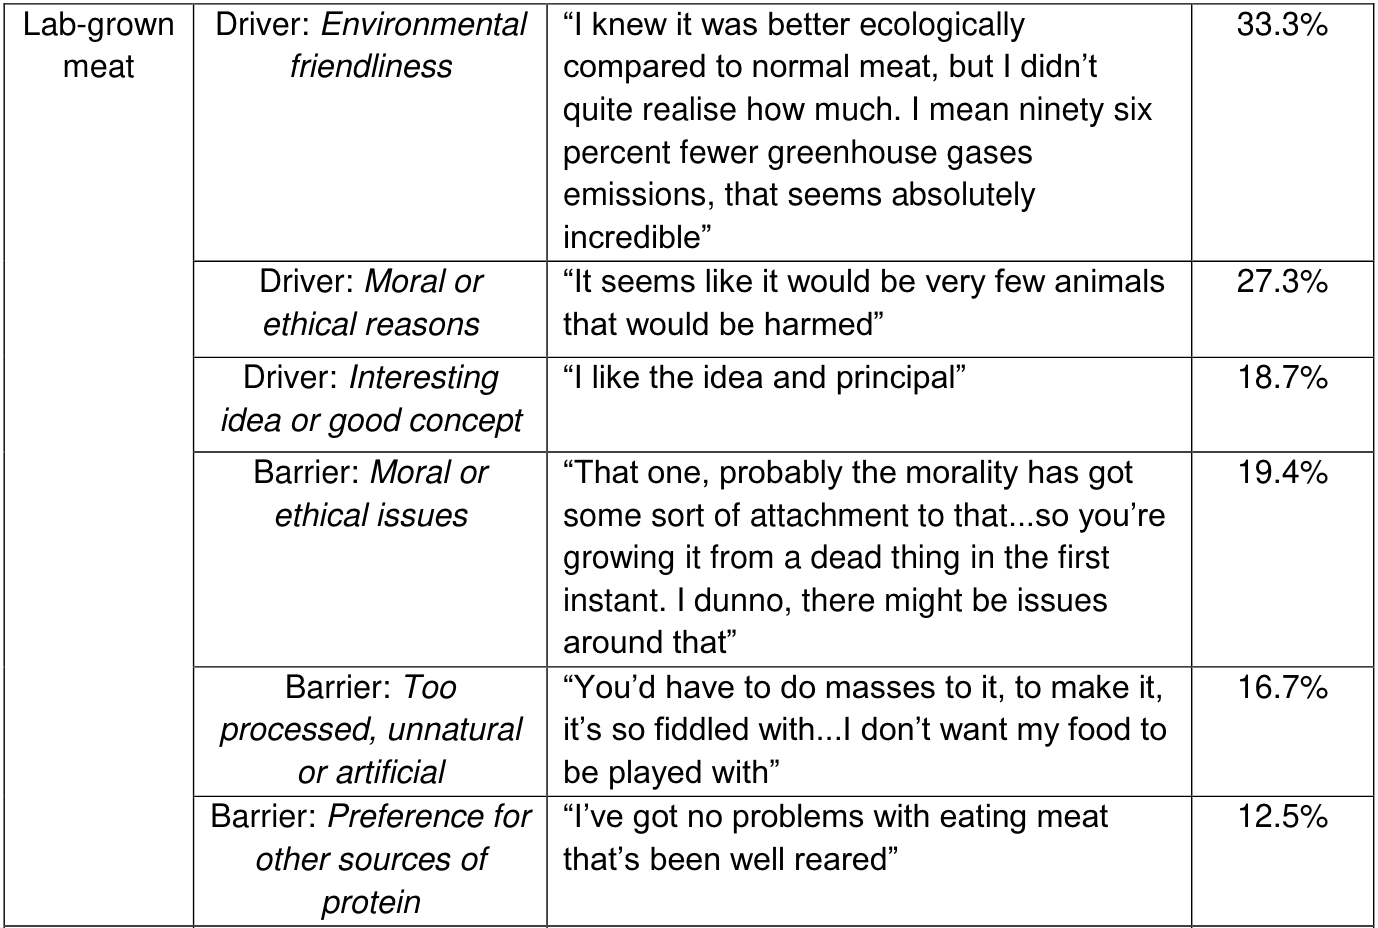
\includegraphics[width=\textwidth]{figures/excerpt-lab-grown-meat.png}
    \caption[Key Personal Drivers and Barriers for Lab-Grown Meat.]{\textbf{Key Personal Drivers and Barriers for Lab-Grown Meat.} This excerpt from Table 1 in \citeauthor{circus_exploring_2018} ’s paper shows the top personal drivers and barriers for lab-grown meat. The drivers are Environmental friendliness, moral/ethical reasons, and interesting ideas (with percentage responses). The barriers are Moral/ethical issues, Too unnatural, and Preference for other proteins with percentages \citep{circus_exploring_2018}.}
    \label{fig:consumer-survey}
  \end{figure}

  As depicted in \autoref{fig:consumer-survey}, recent surveys find that the percentage of consumers currently willing to try cultured meat products spans a wide range, from approximately 10\% on the low end up to 65\% on the high end, with cost, taste, and perceived naturalness being top concerns \citep{bryant_consumer_2018}. However, approximately two-thirds to three-quarters are open to trying lab-grown meat, motivated by potential benefits such as sustainability, animal welfare and health \citep{wilks_attitudes_2017}.

  Demographic factors correlate with acceptance, with younger generations more open to radical food innovations. Urban, liberal, educated consumers also exhibit greater receptiveness to lab-grown meat than rural, conservative and less educated segments \citep{circus_exploring_2018}. Targeting aligned groups can drive early adoption.

  Ongoing consumer research across diverse segments will be invaluable. Conjoint analysis can quantify preferences and willingness-to-pay, while choice modelling examines purchase decisions \citep{wilks_attitudes_2017}. Surveys should track key performance indicators over time.

  These findings will inform educational and promotional initiatives to shift consumer perceptions and build acceptance in retail and food service channels. Monitoring online conversations with semantic analysis tools such as ‘Blue Ocean SWS’ provides real-time insights into evolving attitudes. While scepticism persists in some groups, systematic research and engagement can identify effective strategies for expanding consumer appeal.

  \section{Role of Neuroscience}
  \label{sec:role-of-neuroscience}

  Neuromarketing techniques that measure brain activity provide novel insights into consumer decision-making that can inform efforts to develop and market lab-grown meat.

  Tools like functional magnetic resonance imaging (fMRI) enable researchers to pinpoint specific regions of the brain activated in response to marketing messages or product concepts \citep{bryant_consumer_2018}. This can identify patterns tied to positive or negative perceptions that could potentially be used to refine communication materials.

  Electroencephalography (EEG) detects electrical activity in the brain, helping decipher cognitive processing and emotional engagement with branding elements like logos, names or packaging \citep{khushaba_consumer_2013}. These inputs could guide design choices to spark favourable reactions. However, as is also the case with fMRI, it is essential to note that there may be limitations in broad generalisations due to inherent individual differences in brain structure and function across consumers.

  % TODO Add a figure on neuromarketing techniques

  Biometric measures like galvanic skin response and eye tracking also indicate emotional arousal and attention patterns when consumers view ads or evaluate products \citep{riedl_decade_2020}. This data could help optimise marketing content and formats, such as the choice of words, imagery, and even colour palettes.

  The choice to buy lab-grown meat involves complex risk-benefit calculations that neuroscience can unpack. While consumers are often unaware of their deeper motivations, neuroimaging may reveal unfiltered responses that drive behaviour. Overall, neuromarketing may provide complementary perspectives to traditional consumer research for understanding the psychology behind adopting lab-grown meat. Further research on its specific applications in this context is still needed.

  \section{Marketing Strategies}
  \label{sec:marketing-strategies}

  Marketing lab-grown meat requires strategic and targeted initiatives tailored to consumer segments most likely to adopt this novel product initially. A comparable example targeted tech-savvy early adopters of consumer electronic devices such as the iPhone in 200 \citep{vliert_apple_2021}. As a disruptive innovation, lab-grown meat should first focus on innovators and early adopters who are intrigued by new technologies and exhibit less risk aversion. Engaging these groups helps drive word-of-mouth and advocacy.

  Leveraging social media and partnering with influencers, environmental groups, and technology sites exposes lab-grown meat to aligned audiences receptive to its sustainability and high-tech nature \citep{goodwin_future_2013}. Hashtags and shareable visual content should be part of the social strategy.

  Messaging should focus on safety, nutritional parity with conventional meat, and ecological benefits, as these factors are likely top concerns and motivations \citep{circus_exploring_2018}. The higher production costs can also be framed as premium “clean meat”.

  Monitoring social listening platforms like Reddit and X (formerly Twitter) provides invaluable real-time insight into consumer conversations, questions and attitudes to continually refine communication \citep{verbeke_would_2015}. Viral moments can be capitalised on.

  As production scales and costs decrease, neuromarketing and consumer studies will identify how to pragmatically broaden the appeal of lab-grown meat to the mainstream \citep{verbeke_would_2015}. This may require adjustments to communication and pricing.

  Partnerships with grocery retailers and experiential in-store sampling can help drive the trial and purchase of lab-grown meat products. Retail settings lend themselves to educational efforts about technology and its benefits.

  % TODO Add some imaginary figure on lab-grown meat in a supermarket

  Different branding and positioning may be optimal for launching lab-grown meat in retail channels focused on home cooking versus food service contexts where the experience of eating out differs from preparing one’s meals.

  Just as plant-based alternatives have steadily gained acceptance, employing these targeted marketing strategies based on data-driven insights about early adopters can help establish lab-grown meat as part of the future food system.

  \section{Alternative Benefits of Lab-Grown Meat}
  \label{sec:alternative-benefits}

  Investments in lab-grown meat have the potential to go beyond just producing sustainable food. They can lead to more scientific and engineering innovations due to increased awareness and funding in closely related fields and sub-fields. This can make this industry more attractive for companies to invest in, such as creating better software and hardware, like incubator technologies and nutritional mediums.

  % TODO Add a figure from https://www.nature.com/articles/s41467-021-25236-9

  % TODO Mention and cite this: https://www.frontiersin.org/articles/10.3389/fbioe.2020.00057/full

  Techniques used to culture meat cells promise to revolutionise the creation of complex tissue structures, which, as mentioned in SECTION XYZ, are most likely needed for mass adoption to replace traditional animal-based meat fully and replicate animals’ complex muscle and fat tissues. This has a significantly beneficial side-effect for medical applications, including organ transplants and drug testing models. As a professional working with brain organoids, the author recognises the significant impact that lab-grown meat research could have on developing advanced brain organoid structures. This can benefit neural prosthetics or treatments for neurological disorders by developing more biologically plausible neural tissue as found in vivo. These advancements can enhance cognitive abilities, offer new therapies for patients with severe injuries or degenerative diseases, and benefit the development of more advanced brain-computer interfaces or synthetic biological intelligence.

  Combining topics like food with heart transplantation or brain organoids may initially seem off-putting. However, it is a topic that may arise more frequently as it develops in the coming years.

  \section{Conclusion}
  \label{sec:conclusion}
  Developing and marketing lab-grown meat encompasses an interdisciplinary approach, merging scientific innovation, consumer research, and neuromarketing. This innovative domain addresses sustainable alternatives to conventional animal agriculture and subtly contributes to advancements in related scientific fields.

  The promise of lab-grown meat in addressing environmental and ethical concerns is substantial. However, realising this potential necessitates products that emulate the sensory experience of traditional meat and assure consumers about safety, nutrition, and ecological benefits. Such advancements echo in parallel scientific domains, promising broader technological and health-related impacts.

  Research into consumer perceptions, motivations, and decision-making processes is vital. Marketers can craft strategies that resonate with specific consumer segments by employing quantitative surveys, qualitative studies, and neuromarketing tools. This holistic understanding also informs the broader narrative of innovation and its impact beyond the food industry. From product development to marketing, meticulous attention to taste, texture, nutritional content, safety, and sustainability is essential.

  Transparent branding and labelling are crucial for consumer acceptance and trust, reflecting a commitment to transparency in innovation. Targeted marketing strategies, particularly towards innovators and early adopters, will play a key role in expanding the reach of lab-grown meat. This gradual process, responsive to consumer feedback and effective communication, has the potential to revolutionise global food production and consumption practices.

  \pagebreak
  \singlespacing % No need for double spacing in the references
  \bibliographystyle{references/custom-apa}
  \bibliography{references/bibliography}

\end{sloppypar}
\end{document}’
